\begin{section}{Prueba de concepto}
Para no afectar al funcionamiento de los trabajos que se llevan a cabo en el CITIC, el proyecto se lleva a cabo en un entorno aislado en el cual se despliegan todos los componentes de VCF, con el fin mostrar y probar las capacidades y características de VMware Cloud Foundation. 
El proceso se realizará siguiendo la metodología Scrum, donde en cada ciclo se realizará el despliegue de uno o varios componentes y luego se revisará su configuración y funcionamiento. Primero se instalarán los componentes base de VMware Cloud Foundation\footnote{Los componentes base de VCF son VMware vSphere, VMware vSAN y VMware NSX-T} usando el programa VMware Lab Constructor (VLC) v4.0.1\footnote{Herramienta que permite crear un generar de forma automatizada un entorno embebido para probar las funcionalidades de VMware Cloud Foundation.}. Posteriormente se instalarán los componentes suite VMware vRealize orientados a la gestión de usuarios del SDDC y a proporcionar un servicio de aprovisionamiento privado, llamados Workspace One Access y vRealize Automation respectivamente. Finalmente, se comprobará el funcionamiento general del SDDC y las posibilidades que ofrece el servicio Cloud construido.

\begin{subsection}{Preparación}
  En esta sección se describe como se prepara el entorno de pruebas con los elementos y servicios utilizados para realizar el despliegue de la solución y necesarios para su correcto funcionamiento.

  \begin{subsubsection}{VMware Lab Constructor v4.0.1}
    El programa VMware Lab Constructor v4.0.1 (VLC), es una herramienta desarrollada por trabajadores de VMware, la cual permite crear un entorno embebido dentro del host utilizado como entorno de pruebas. Este entorno se compone de cuatro hosts con el hipervisor ESXi en forma de VMs. Dentro de estos hosts, VLC despliega los componentes de VCF.

    \begin{figure}[h!]
      \centering
      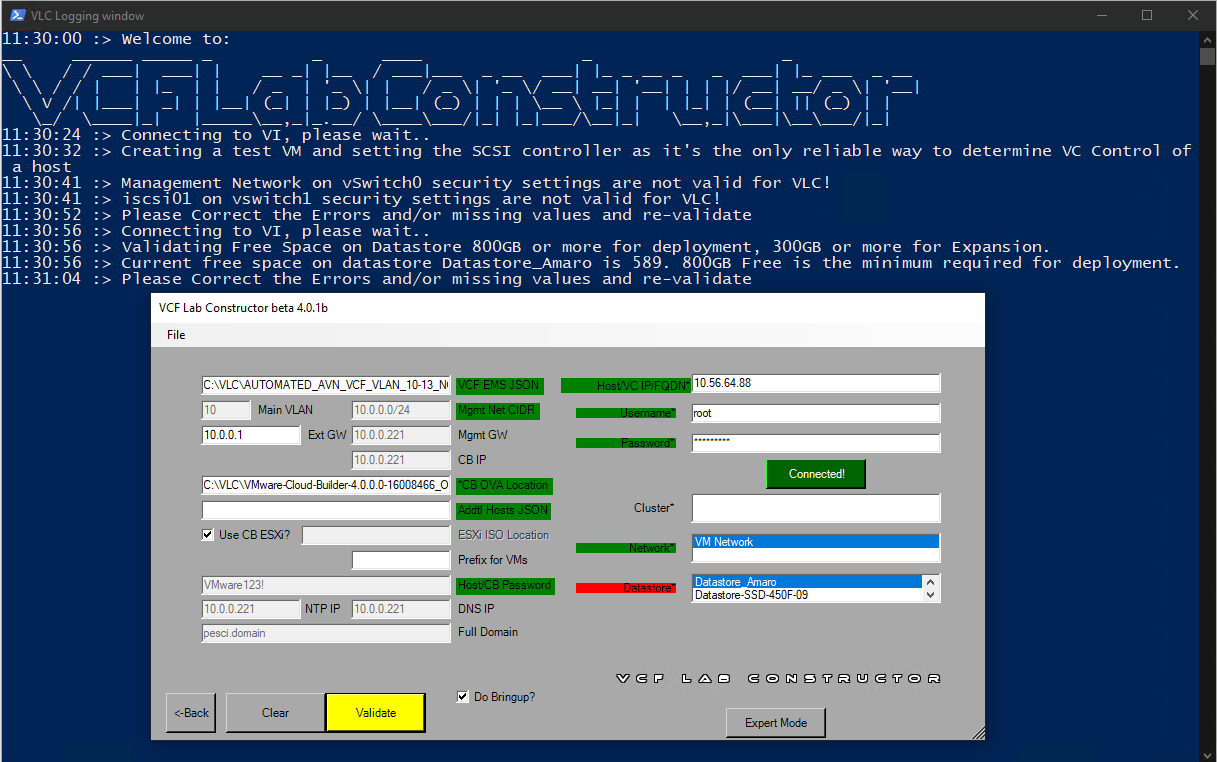
\includegraphics[width=0.8\textwidth]{imaxes/pruebaconcepto/VLC.png}
      \caption{Herramienta VMware Lab Constructor v4.0.1b}
      \label{fig:VLC}
    \end{figure}
    \FloatBarrier

  \end{subsubsection}

  \begin{subsubsection}{Host ESXi}  
    El host sobre el que VLC realiza la instalación del entorno se trata de un servidor con el hipervisor ESXi instalado. Este servidor cuenta con una memoria RAM de 192 GB, una CPU de 28,8 GHz y está conectado a un datastore formado por discos SSD y con una capacidad de 3 TB. Además, incorpora dos interfaces de red. La primera interfaz se conecta a una red para acceder al datastore, mientras que la segunda, representada con el nombre \textit{vmnic0} en la figura \ref{fig:estructura-generada-por-VLC}, se conecta a una red utilizada para acceder de forma remota al servidor y a otra red dedicada a comunicar los componentes desplegados dentro del host.

    % Como base para la instalación se utiliza un servidor físico con el hipervisor ESXi instalado. Este host se utiliza para desplegar los componentes de VMware Cloud Foundation para crear un pequeño SDDC embebido para probar sus funciones. Este host cuenta con una memoria RAM de 192 GB, una CPU de 28,8 GHz y un \textit{datastore} con discos SSD con 2 TB de capacidad. Cuenta con dos interfaces físicas, una que conecta al host con el \textit{datastore} y otra a la que se conectan dos redes, una llamada \textit{Management Network} que permite acceder al host desde una VM para gestionarlo, y otra llamada \textit{VM Network} donde se conectan todas las VMs generadas por VLC y de los servicios que dan soporte a los componentes de VMware Cloud Foundation.
  \end{subsubsection}

  \begin{subsubsection}{Servicios}
    Los servicios externos requeridos por VCF se sitúan dentro del mismo servidor físico. Estos están colocados en una VM con el sistema operativo Windows Server 2016, el cual incluye DNS, NTP, SMTP, y los servicios Active Directory (AD) y Certificate Authority (CA). También incorpora un router en forma de VM con el sistema operativo VyOS, que además cuenta con servicio DHCP. El servidor DNS utiliza \textit{pesci.domain} como nombre de dominio. El almacén Active Directory sustituye al directorio de usuarios de la UDC para poder manejar cuentas de usuarios sin causar conflictos en el funcionamiento de los servicios en producción.
    % Todos los servicios requeridos por VMware Cloud Foundation se despliegan sobre el mismo servidor en forma de VMs. Una de las VMs es Windows Server 2016 que contiene un servidor DNS, un servidor NTP, un servidor Active Directory, un servidor SMTP y ejerce también como Certificate Authority. Otra VM contiene el sistema operativo VyOS que funciona como un router virtual y como servidor DHCP. Una última VM con Windows 10\footnote{Se refiere a ella como \textit{Jump Host}.} se requiere para ejecutar VLC y acceder al entorno embebido generado por VLC.
    % El servidor DNS contiene el nombre y su respectiva dirección que un componente de VCF utilizará para que sus instancias se puedan comunicar con otras. Este servidor DNS implementa un único dominio que se denomina \textit{pesci.domain}. El servidor Active Directory proporciona un almacén de usuarios y grupos de usuarios a los cuales se les configura un rol dentro de cada componente de SDDC. Se utiliza este repositorio de usuarios en lugar del directorio real de la UDC para evitar posibles problemas del servicio. El router VyOS tiene configuradas todas las subredes y VLANs que VMware Cloud Foundation utiliza en la capa L3 de la infraestructura física y proporciona acceso a Internet, en las cuatro interfaces que conectan con las instancias de VMware NSX-T Edge utiliza enrutamiento dinámico BGP. El servidor DHCP se utiliza para asignar una dirección IP a las interfaces Tunnel EndPoint (TEP)\footnote{Más adelante se describirá la función de este elemento} de cada host ESXi.    
  \end{subsubsection}
  \begin{figure}[h!]
    \centering
    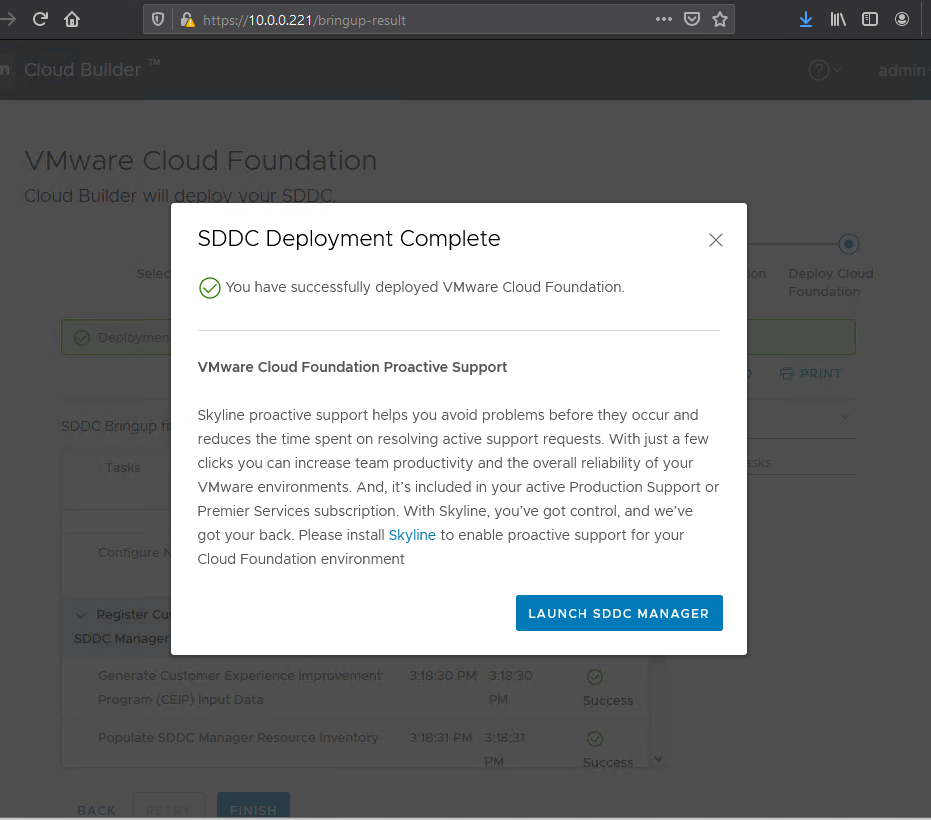
\includegraphics[width=0.7\textwidth]{imaxes/pruebaconcepto/fin-despliegue.png}
    \caption{Finalización del despliegue inicial de VMware Cloud Foundation.}
    \label{fig:fin-despliegue}
  \end{figure}
  \FloatBarrier
    \begin{figure}[h!]
      \centering
      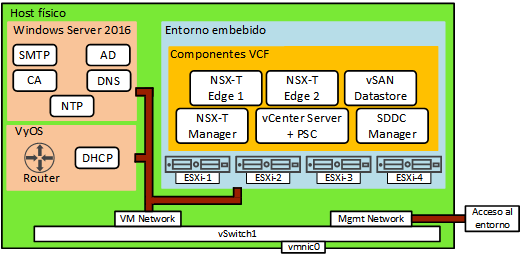
\includegraphics[width=0.8\textwidth]{imaxes/pruebaconcepto/hostFisico.png}
      \caption{Servicios desplegados y entorno embebido generado por VLC dentro del host físico.}
      \label{fig:estructura-generada-por-VLC}
    \end{figure}
    \FloatBarrier
    Una vez finalizado el despliegue como se muestra en la figura \ref{fig:fin-despliegue}, el entorno embebido generado con VLC dentro del host físico, incluyendo las VMs de los componentes de VCF y los servicios necesarios para su correcto funcionamiento, se muestra en la figura \ref{fig:estructura-generada-por-VLC}. Esta figura también incluye las dos redes a las que se conecta la interfaz \textit{vmnic0} del host. \textit{VM Network} comunica a todos los elementos desplegados y representa la red física del entorno. La red \textit{Mgmt Network} se utiliza para acceder al host de forma remota.
    % \begin{figure}[h]
    %   \centering
    %   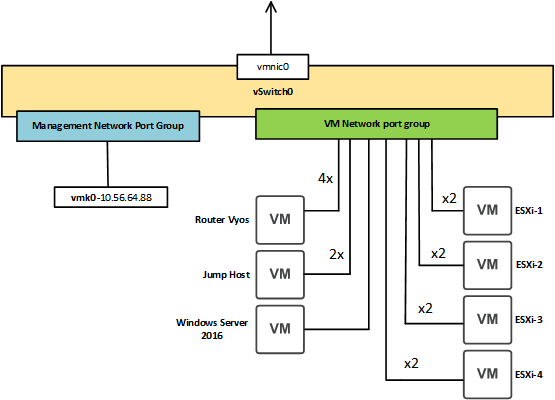
\includegraphics[width=0.6\textwidth]{imaxes/pruebaconcepto/vSwitch0HostFisico.png}
    %   \caption{Máquinas virtuales en el host físico.}
    %   \label{fig:VMs-alojadas-host-fisico}
    % \end{figure}
    % \FloatBarrier

    % En la imagen anterior se muestran las VMs que están funcionando sobre el host físico y que representan los componentes de la infraestructura física de un SDDC real, junto con el número de interfaces que se utilizan en cada una. Cada host ESXi generado por VLC cuenta con dos interfaces de red. El router VyOS, Jump Host y Windows Server 2016 se configuran antes del despliegue de VMware Cloud Foundation con VLC y se comunican con el entorno generado por VLC a través del \textit{port group} VM Network. El \textit{port group} Management Network se utiliza para acceder a la configuración del host físico a través de la dirección IP que se indica. Se utiliza la interfaz vmnic0 del host como salida del tráfico generado por el vSwitch0.
    % \FloatBarrier

    % \begin{figure}[h]
    %   \centering
    %   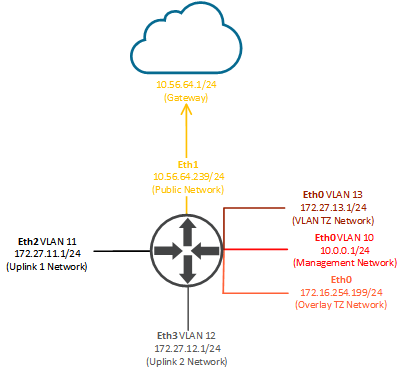
\includegraphics[width=0.4\textwidth]{imaxes/pruebaconcepto/RouterFisicoL3.png}
    %   \caption{Interfaces del router Vyos.}
    %   \label{fig:interfaces-router-fisico-L3}
    % \end{figure}
    % \FloatBarrier

    % En la imagen anterior se muestra la configuración del router VyOS. Cada una de las interfaces se debe configurar antes del despliegue de VCF. Todas usan MTU de 9000 Bytes ya que la mayoría de componentes de VCF utilizan paquetes de red \textit{jumbo frame}. En las interfaces Eth2 y Eth3 el router utiliza enrutamiento dinámico BGP donde el AS local es 65001 y el AS remoto es AS 65003, configurado para anunciar a sus vecinos la red 10.0.0.0/24 Management Network. Las direcciones configuradas como \textit{neighbour} son: 172.27.11.2, 172.27.11.3, 172.27.12.2 y 172.27.12.3. En la dirección IP 172.27.254.199 de la interfaz eth0, el router proporciona un servidor DHCP que asigna direcciones IP en el rango 172.16.254.0 - 172.16.254.100.
    % \FloatBarrier

    % \begin{figure}[h]
    %   \centering
    %   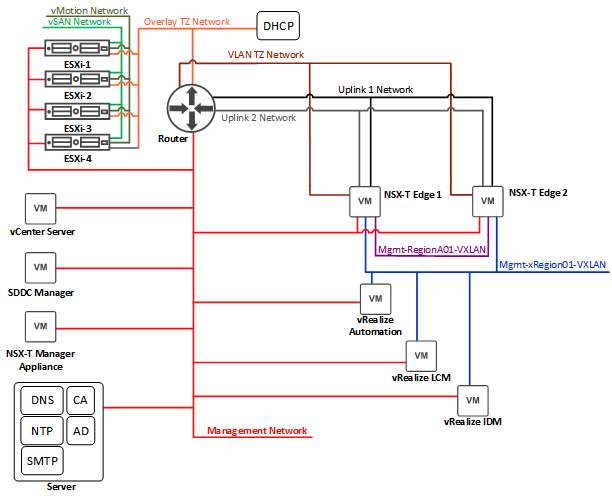
\includegraphics[width=0.6\textwidth]{imaxes/pruebaconcepto/RedDesdeDentro.png}
    %   \caption{Topología de las redes del entorno desplegado.}
    %   \label{fig:red-L3-infraestructura-fisica}
    % \end{figure}
    % \FloatBarrier

    % En la imagen anterior se muestran todos los componentes de VMware Cloud Foundation desplegados por VLC y los desplegados posteriormente para completar los objetivos del proyecto, como se conectan con los distintos servicios de red y a que redes se conectan. Las redes Mgmt-xRegion01-VXLAN y Mgmt-Region01A-VXLAN se corresponden a redes virtuales gestionadas por VMware NSX-T que no requieren ninguna configuración adicional en la capa 3 de la infraestructura física (esto se verá con detalle en el apartado de diseño de VMWare NSX-T).
    % \FloatBarrier
  \end{subsection}

\begin{subsection}{Diseño y configuración del Management Domain}
\input{contido/metodoloxia/pruebaconcepto/diseñovSphere}
\input{contido/metodoloxia/pruebaconcepto/diseñoNSX-T}
\end{subsection}
\begin{subsection}{Operaciones de la Arquitectura}
    El entorno ya está configurado para funcionar como un SDDC, a partir de este punto ya no es necesario realizar ninguna modificación en la infraestructura física ya que todas las tareas que se deben realizar están dentro del alcance de los componentes de VMware Cloud Foundation. Para finalizar la construcción del SDDC y habilitar un servicio donde los usuarios puedan aprovisionar recursos bajo demanda, se instalarán sobre el entorno desplegado las aplicaciones Workspace ONE Access \footnote{VMware vRealize Identity Manager} (WSA) y VMware vRealize Automation (vRA). La primera permite al administrador conectar con el servidor de usuarios Active Directory y gestionarlos para proveer un servicio de autenticación centralizado a múltiples aplicaciones como VMware vRealize Automation. La segunda aplicación permite a los usuarios aprovisionar recursos de forma automatizada desde un catálogo de recursos. VMware vRealize Suite Licfecycle Manager (vRSLCM) es el componente que permite administrar vRA y WSA, su instalación y actualizaciones, las contraseñas de administrador y sus certificados, para ello necesita comunicarse con VMware vCenter Server. Se desplegará una instancia de cada componente en el \textit{management domain} creado anteriormente y estarán conectadas al \textit{segment}/subred \textit{Mgmt-xRegion01-VXLAN}.
    
    % \begin{subsubsection}{vRealize Suite Lifecycle Manager}
        
    % \end{subsubsection}
    \begin{subsubsection}{Workspace One Access}
        Los usuarios que necesiten acceder a vRA deben estar registrados en el directorio de Workspace One Access. Este componente centraliza el acceso de todos los productos de VMware vRealize. Cuando se despliega se debe configurar un Active Directory que en el caso del entorno está situado en la VM con Windows Server 2016. Dentro del Active Directory existen grupos de seguridad y perfiles de usuario, un perfil de usuario contiene información como nombre, apellidos, dirección e-mail, nombre de usuario y contraseña\footnote{Se pueden configurar más campos pero los que se describen son los obligatorios a la hora de crear un usuario.}, y este puede formar parte de varios grupos de seguridad. Una vez configurado, cada aplicación se conectará a WSA y se podrán asignar roles para los grupos de seguridad y usuarios estableciendo así un nivel de acceso. Además, cada usuario registrado tendrá disponible un catálogo de aplicaciones en el portal de WSA cuyo administrador establecerá que aplicaciones están habilitadas para cada usuario o grupo, eso sí, para que el usuario pueda acceder a ella previamente se debe establecer un rol para ese usuario dentro de la aplicación.

        %*****USUARIOS QUE HAY EN EL ENTORNO Y EL ACCESO A CADA APLICACIÓN*******%
        \begin{figure}[h]
            \centering
            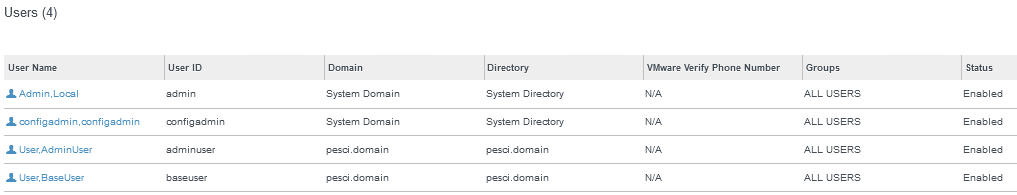
\includegraphics[width=0.4\textwidth]{imaxes/vRealize_pruebaconcepto/usuariosDefinidos.png}
            \caption{Muestra los usuarios definidos en el Active Directory sincronizados en Workspace One Access.}
            \label{fig:users-defined-AD}
        \end{figure}
        \FloatBarrier
        En la Figura \ref{fig:users-defined-AD} se muestran los dos usuarios definidos en el Active Directory y dos usuarios que se corresponden a los perfiles de administración de WSA, no se utilizarán grupos de seguridad para reducir la complejidad pero su configuración en las aplicaciones de VMware es igual que para los perfiles de usuario. En un entorno real existen usuarios que controlan a otros usuarios y establecen su nivel de acceso, a parte de los perfiles de administrador de cada aplicación. Para el entorno se define el perfil \textit{adminuser} que será el encargado de gestionar el acceso de dos usuarios (\textit{baseuser1} y \textit{baseuser2}) que serán los que consuman a las aplicaciones desplegadas (vRSLCM y vRA). El primero tendrá acceso y permisos de edición en las aplicaciones vRSLCM y vRA, mientras que los dos usuarios base solo podrán acceder a vRA y dentro de este el usuario admin definirá que servicios están habilitados para cada uno.

        %************************************************************************%

    \end{subsubsection}

    \begin{subsubsection}{VMware vRealize Automation}
        El punto a través del cual los usuarios pueden aprovisionar sus recursos es vRealize Automation. Este producto provee el servicio cloud. 
        \begin{figure}[h]
            \centering
            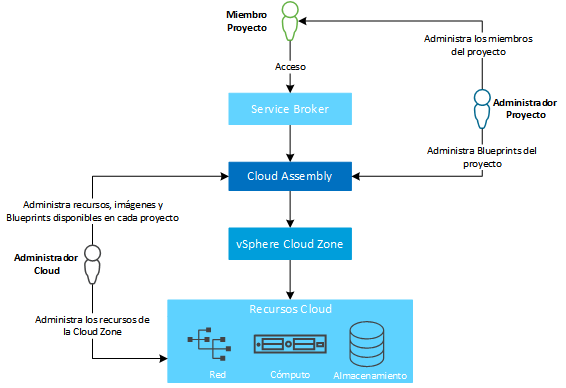
\includegraphics[width=0.8\textwidth]{imaxes/vRealize_pruebaconcepto/ComponentesVRA.png}
            \caption{Componentes de VMware vRealize Automation y tareas que realiza cada rol de usuario.}
            \label{fig:users-defined-AD}
        \end{figure}
        \FloatBarrier
        Internamente vRA se divide en varios servicios que permiten gestionar los diferentes aspectos de la cloud. Para centrarse en los objetivos de este proyecto solo se hace referencia a dos de esos servicios, el primero es Cloud Assembly el cual permite administrar la infraestructura disponible controlar el uso que se hace de esos recursos, y el segundo es Service Broker, utilizado por los usuarios para aprovisionar los recursos desde un catálogo de plantillas. La obtención de los recursos por parte del usuario se hace desplegando una serie de plantillas llamadas Blueprints diseñadas previamente, en donde se define un conjunto de VMs y recursos de red y de almacenamiento incluyendo otros aspectos como la configuración de cada uno de los recursos, como redes de la infraestructura que se utilizan, cantidad de almacenamiento, o la ubicación del despliegue en la infraestructura. Son ficheros de código con extensión \textit{.yaml} donde se indican etiquetas, aunque también se pueden diseñar con un editor gráfico. Estas plantillas están relacionadas con proyectos, una plantilla pertenece a uno o varios proyectos donde existe un coordinador de proyecto que se encarga de diseñar Blueprints y de administrar los usuarios miembros de ese proyecto. Los proyectos de vRA permiten limitar los recursos para que un conjunto de usuarios pueda desplegar los componentes definidos en las Blueprints disponibles, como la cantidad de memoria RAM, cantidad de instancias que se pueden desplegar y cantidad de almacenamiento, también aquellas redes que se pueden utilizar. Desde el punto de vista de vRA, la infraestructura se divide en Cloud Zones, las cuales son conjuntos de recursos situados en distintos proveedores Cloud que pueden ser públicos como AWS o Azure, o privados que solo pueden ser clusters vSphere. En el caso del entorno desplegado solo se tendrá una única Cloud Zone de tipo vSphere. En cada Cloud Zone se define como se deben distribuir los recursos aprovisionados sobre la infraestructura. 
        Finalmente será el administrador de la infraestructura el que se encargue de proveer los recursos, administrar los proyectos disponibles, gestionar los coordinadores de cada proyecto y controlar y limitar el uso de los recursos.
        % Finalmente, vRA permite configurar tarjetas donde se puede definir el coste del aprovisionamiento de CPU, almacenamiento y memoria RAM, además del coste de uso de otros elementos como sistemas operativos, el uso de una determinada red o el uso de una determinada Cloud Zone. Estas tarjetas se asignan por proyecto para determinar el coste que tendrá el consumo de recursos por mes.


    \end{subsubsection}

    
\end{subsection}
\end{section}